%%%%%%%%%%%%%%%%%%%%%%%%%%%%%%%%%%%%%%%%%%%%%%%%%%%%%%%%%%%%%%%%%%%%%
%
%  This is a sample LaTeX input file for your contribution to 
%  the MC2013 conference. Modified by R.C. Martineau at INL from A. 
%  Sood at LANL, from J. Wagner ORNL who obtained the original class 
%  file by Jim Warsa, LANL, 16 July 2002}
%
%  Please use it as a template for your full paper 
%    Accompanying/related file(s) include: 
%       1. Document class/format file: mc2013.cls
%       2. Sample Postscript Figure:   figure.eps
%       3. A PDF file showing the desired appearance: template.pdf 
%    Direct questions about these files to: richard.martinea@inl.gov
%
%    Notes: 
%      (1) You can use the "dvips" utility to convert .dvi 
%          files to PostScript.  Then, use either Acrobat 
%          Distiller or "ps2pdf" to convert to PDF format. 
%      (2) Different versions of LaTeX have been observed to 
%          shift the page down, causing improper margins.
%          If this occurs, adjust the "topmargin" value in the
%          mc2013.cls file to achieve the proper margins. 
%
%%%%%%%%%%%%%%%%%%%%%%%%%%%%%%%%%%%%%%%%%%%%%%%%%%%%%%%%%%%%%%%%%%%%%


%%%%%%%%%%%%%%%%%%%%%%%%%%%%%%%%%%%%%%%%%%%%%%%%%%%%%%%%%%%%%%%%%%%%%
\documentclass{ansconf}
%
%  various packages that you may wish to activate for usage 
\usepackage{graphicx}
\usepackage{tabls}
\usepackage{hyperref}
%

%General Short-Cut Commands
\newcommand{\superscript}[1]{\ensuremath{^{\textrm{#1}}}}
\newcommand{\subscript}[1]{\ensuremath{_{\textrm{#1}}}}
%\newcommand{\nuc}[2]{\superscript{#2}{#1}}
\newcommand{\nuc}[2]{{#1}{#2}}
\newcommand{\ith}[0]{$i^{\mbox{th}}$ }
\newcommand{\jth}[0]{$j^{\mbox{th}}$ }
\newcommand{\kth}[0]{$k^{\mbox{th}}$ }
\newcommand{\us}[0]{$\mu$s }

% New definition of square root:
% it renames \sqrt as \oldsqrt
\let\oldsqrt\sqrt
% it defines the new \sqrt in terms of the old one
\def\sqrt{\mathpalette\DHLhksqrt}
\def\DHLhksqrt#1#2{%
\setbox0=\hbox{$#1\oldsqrt{#2\,}$}\dimen0=\ht0
\advance\dimen0-0.2\ht0
\setbox2=\hbox{\vrule height\ht0 depth -\dimen0}%
{\box0\lower0.4pt\box2}}



% Insert authors' names and short version of title in lines below
%
\authorHead{Anthony M. Scopatz}
\shortTitle{First \& second order approximations to stage numbers in
            multicomponent enrichment cascades}

\confTitle{International Conference on Mathematics and Computational Methods
  Applied to Nuclear Science \& Engineering (M\&C 2013)}
\confLocation{Sun Valley, Idaho, USA, May 5-9, 2013}
\confPublished{on CD-ROM, American Nuclear Society, LaGrange Park, IL (2013)}

%%%%%%%%%%%%%%%%%%%%%%%%%%%%%%%%%%%%%%%%%%%%%%%%%%%%%%%%%%%%%%%%%%%%%
%
%   BEGIN DOCUMENT
%
%%%%%%%%%%%%%%%%%%%%%%%%%%%%%%%%%%%%%%%%%%%%%%%%%%%%%%%%%%%%%%%%%%%%%
\begin{document}

\title{FIRST \& SECOND ORDER APPROXIMATIONS TO STAGE NUMBERS IN 
       MULTICOMPONENT ENRICHMENT CASCADES}

\author{Anthony Scopatz}
\affil{The University of Chicago\\
  5754 S. Ellis Ave, Chicago, IL, 60637 \\
  scopatz@flash.uchicago.edu}

\maketitle

\begin{abstract}
\raggedright
Some Abstract text.

\emph{Key Words}: multicomponent, enrichment, symbolic, PyNE
\end{abstract}

\section{Introduction}
\label{sec:intro}

The matched abundance ratio cascade (MARC) equations calculate the concentrations
and flow rates through a multicomponent enrichment cascade contain. These may
be solved either using standard numeric optimizers or by using a symbolic 
expression library.  The advantage of using a symbolic library is that the 
representation of the MARC equations looks very similar to its mathematical form.
The disadvantage is that, without a compilation or code generation step, symbolic 
libraries tend to be significantly more computationally intensive.  In a related 
study upon which this paper is based, code generation was used and the symbolic
solution was found to be 20 - 300 times faster than a standard numeric solver.
An ecosystem of symbolic mathematics software tools are available: 
Mathematica \cite{Wolfram2008}, Maple \cite{Maple16},  Maxima \cite{Maxima5}, 
and SymPy \cite{SymPy2012}.  

The MARC equations for multicomponent separations were originally formulated 
by de la Garza \cite{DelaGarza1969}.
An example implementation of a constrained numerical optimizer solution may be 
found in PyNE and elsewhere \cite{pyne:enrichment,doi:10.1080/01496391003793884}.  
Alternatively, a symbolic implementation may also now be found in PyNE.  The symbolic
version uses variable substitution and elimination to reduce the system to one 
equation and one unknown.

However, when reducing systems by variable elimination, closed form expressions for 
all independent variables are required.  For some indpendent variables this is 
relatively easy to acomplish. For others, such as the number of product stages in
a cascade, it may be shown that no closed form solution is possible.  In such cases 
the strategy is to derive a closed form approximation for this independent variable.

What form this approximation takes and how accurate it needs to be are dependent on 
the actual system of equations being examined.  For MARC and the number of product
stages, a Taylor series approximation was used.  Both first and second order 
approximations are explored here.  In terms of computation efficiency, lower order 
approximations are desirable.  However, increased order may be required to 
satisfactorily be able to solve the system of equations.

This paper proceeds as follows.  The symbolic methodology 
is discussed in \S\ref{sec:meth}.  This includes an overview of the
MARC equations, a description of the symbolic strategy, and the
derivation of both first and second order approximations.
The results of the Tayor series approximations are then presented in \S\ref{sec:res}. 
Lastly, \S\ref{sec:conc} discusses the validity of each approximation and other
possible approximation schemes.

\section{Symbolic Methodology}
\label{sec:meth}
At its core, the solution to coupled multicomponent enrichment cascade equations is
a minimization problem \cite{Wood1999}.  In a matched abundance ratio 
\cite{DelaGarza1969} cascade this may be cast as the minimization of 
the total flow rate $L$ through the cascade normalized by the feed flow rate $F$.  
Thus, the positive and unitless optimization variable $L/F$ is formed.  Traditionally, 
minimizing this parameter as a function of other cascade state variables has been 
performed either via off-the-shelf optimization libraries 
\cite{doi:10.1080/01496391003793884} or custom built solvers \cite{PyNE2012}.

However, both of these approaches rely on writing code idiomatic to the underlying 
programming language.  For example, many numerical constraint optimizers, in order 
to handle the case of arbitrarily complex expressions, accept as their primary 
argument a function object or pointer.  Then for every iteration the optimizer must 
call the function whose inputs are to be optimized.  This involves (in compiled 
languages) setting up a new stack and allocating new memory for every solver 
iteration.  While good 
optimizers will be efficient in terms of the number of function calls they make, 
there is no way for them to avoid multiple function calls and remain sufficiently 
general. The number of function calls that are needed scales \emph{at least} linearly 
with the number of equations in the system.

On the other hand, if it is possible to convert the system of equations 
into a single expression -- no matter how complicated -- then the problem has been 
recast into the optimization of a single function over a single variable.   This 
may be easily handed off to any number of well known algorithms, such as Newton's
method, the secant method, or the bisection method.  In such a form, the solution 
will have a vastly reduced computational overhead as compared to standard 
numerical solvers. 

Naturally, performing the above variable substitution and elimination to obtain a 
single expression is difficult in many cases and mathematically impossible in most 
others.  For MARC systems, as is shown in \S \ref{sec:symes}, reduction of $L/F$
to a single expression is possible.

Rather than phrasing this as a numerical optimization problem from the start, the 
opposite conceptual tactic is taken.  The MARC system is expanded, manipulated, 
and substituted symbolically during the majority of the calculation.  The actual 
numerical results of the calculation are only computed as needed at the final step.
Symbolic manipulations are concluded prior to compilation, resulting in 
very fast run time solutions.

In \S \ref{sec:marceq} the standard MARC system of equations is detailed. 
Then the novel reinterpretation of the MARC equations is related in 
\S \ref{sec:symes}.  
Lastly, \S \ref{sec:codegen} characterizes the pipeline that takes the symbolic MARC 
equations and converts them into fast machine code.  
For the remainder of \S \ref{sec:meth}, a three-component natural uranium fed 
cascade will be used when example data is required.
Cascades with a greater numbers of components will be discussed in \S \ref{sec:res}.

\subsection{The MARC Equations}
\label{sec:marceq}

The method to compute matched abundance ratio cascades has been 
previously described in other sources, from de la Garza in the
1960s. This method is explained here in order to build up to the symbolic first and 
second order approximations that will be seen.
For more information please refer to de la Garza
\cite{DelaGarza1969}, von Halle \cite{VonHalle1987}, Wood \cite{Wood1999}, 
Song \cite{doi:10.1080/01496391003793884}, or the symbolic methodology on which this 
work is based \cite{Scopatz2012}.

Set $N$ the total number of stages in an enrichment cascade, $N_P$ as the number of 
product stages above the feed entry point, and $N_T$ as the number of tails
stages.  Thus,
\begin{equation}
N = N_P + N_T
\end{equation}
MARC needs a special nuclide to also be set such that it is enriched in the 
product (subscript P).  This is called the first key component, $j$.  
There is also be a second key component, $k$, from which $j$ is 
separated. Therefore $k$ can be said to be enriched in the tails stream (subscript T).

The overall stage separation factor $\alpha$ [unitless] is the per mass 
enrichment ratio from one stage to the next.  From $\alpha$ 
stage separation factors for individual nuclides may be computed. 
These are called $\beta_i$ for the \ith component of a mixture $I$ and are 
computed by:
\begin{equation}
\beta_i = \alpha^{M^* - M_i}
\label{beta_i}
\end{equation}
$M_i$ is the molecular weight [amu] of the \ith
nuclide while $M^*$ [amu] is a flow rate optimization parameter.  An initial
guess for 
$M^*$ is normally set by the average of the molecular weights of the key components. 
Using the subscript $0$, denote the initial guess by $M_0^*$:
\begin{equation}
M_0^* = \frac{1}{2}\left(M_j + M_k\right)
\label{mstar-guess}
\end{equation}
Also the constraint $M_j < M_k$ is applied when picking the order for$j$ \& $k$.
Thus $M^*$ is bounded on the range $M^*\in[M_j,M_k]$ when minimizing $L/F$.

Call $F$, $P$, and $T$ the feed, product, and tails mass flow rates subject to 
the conservation equation,
\begin{equation}
F = P + T
\label{total-flow-constraint}
\end{equation}
Also have $x$ as a normalized mass concentration vector such that $x_i^F$, 
$x_i^P$, $x_i^T$ are the concentrations of the \ith nuclide of the feed, product,
and tails.  From here:
\begin{equation}
1 = \sum_i^I x_i^F = \sum_i^I x_i^P = \sum_i^I x_i^T 
\end{equation}
The flow rate ratios are seen as follows:
\begin{equation}
\frac{P}{F} = \sum_i^I x_i^F\frac{\beta_i^{N_T+1} - 1}
                                 {\beta_i^{N_T+1} - \beta_i^{-N_P}}
\label{ppf-full}
\end{equation}
\begin{equation}
\frac{T}{F} = \sum_i^I x_i^F\frac{1 - \beta_i^{-N_P}}
                                 {\beta_i^{N_T+1} - \beta_i^{-N_P}}
\label{tpf-full}
\end{equation}
Equations \ref{ppf-full} \&  \ref{tpf-full} are then reduced to functions
of just $j$ for an ideal cascade.
\begin{equation}
\frac{P}{F} = \frac{x_j^F - x_j^T}{x_j^P - x_j^T}
\label{ppf-key}
\end{equation}
\begin{equation}
\frac{T}{F} = \frac{x_j^F - x_j^P}{x_j^T - x_j^P}
\label{tpf-key}
\end{equation}

Equations \ref{ppf-full} \& \ref{tpf-full} or equations \ref{ppf-key} \& 
\ref{tpf-key} both allow for the calculation of the \ith component concentrations in 
the product and tails as a function of the feed concentrations.
\begin{equation}
x_i^P = \frac{x_i^F}{\frac{P}{F}}\cdot\frac{\beta_i^{N_T+1} - 1}
                                           {\beta_i^{N_T+1} - \beta_i^{-N_P}}
\label{prod-concentration}
\end{equation}
\begin{equation}
x_i^T = \frac{x_i^F}{\frac{T}{F}}\cdot\frac{1 - \beta_i^{-N_P}}
                                           {\beta_i^{N_T+1} - \beta_i^{-N_P}}
\label{tail-concentration}
\end{equation}
However, the component nuclides themselves are
also subject to mass conservation:
\begin{equation}
x_i^FF = x_i^PP + x_i^TT
\label{comp-flow-constraint}
\end{equation}

By their name, MARCs require that at every stage any two flows of 
the same type ($F$, $P$, \& $T$) must have the same relative concentrations of 
$j$ \& $k$.  Thus, say that $R$ is an abundance ratio.  For matched abundance 
ratio cascades, 
\begin{equation}
R^F = \frac{x_j^F}{x_k^F}; \;\;\; R^P = \frac{x_j^P}{x_k^P}; \;\;\; 
R^T = \frac{x_j^T}{x_k^T}
\label{abund_ratios}
\end{equation}
The ratios in these equations are valid for all stages in the cascade.

Lastly, the total flow rate per $F$ for a cascade is computed as follows:
\begin{equation}
\frac{L}{F} = \sum_i^I \frac{\frac{P}{F}x_i^P\ln(R^P) + \frac{T}{F}x_i^T\ln(R^T) 
                                                      - x_i^F\ln(R^F)}
                            {\ln(\beta_j)\frac{\beta_i - 1.0}{\beta_i + 1.0}}
\label{ltot-over-feed}
\end{equation}
Equation \ref{ltot-over-feed} is minimized when computing the `optimal' cascade.
This is analogous to the $L/P$ expression found in \cite{Wood1999}.

Typically, the following cascade parameters are known:
$\alpha$, 
$j$, $k$, 
$M_i$ for all $i\in I$, 
$x_i^F$ for all $i\in I$, 
the key product enrichment $x_j^P$, and the key 
tails enrichment $x_j^T$.  Therefore the optimized cascade is given by 
a system of three equations and three unknowns --
$N_P$, $N_T$, and $M^*$ -- and is therefore well determined.
\begin{equation}
\frac{x_j^P}{x_j^F}\cdot\frac{P}{F} - \frac{\beta_j^{N_T+1} - 1}
                                           {\beta_j^{N_T+1} - \beta_j^{-N_P}} = 0
\label{prod-constraint}
\end{equation}
\begin{equation}
\left(\frac{x_j^F}{\frac{T}{F}} \cdot \frac{1 - \beta_i^{-N_P}}
                                           {\beta_j^{N_T+1} - \beta_j^{-N_P}} \right)
- \left(x_j^T\cdot\sum_i^{I} x_i^T\right) = 0
\label{tail-constraint}
\end{equation}
\begin{equation}
\min\left[\frac{L}{F}\right]\to \frac{d}{dM^*} \frac{L}{F} = 0
\label{minlt-constraint}
\end{equation}
Equation \ref{prod-constraint} is a rearrangement of equation \ref{prod-concentration}
when evaluated for the second key component.
Equation \ref{tail-constraint} is gained by equations \ref{tpf-full} \&
\ref{tail-concentration} when evaluated for the second key component.
Equation \ref{minlt-constraint} comes from the extreme value theorem of calculus
and equation \ref{ltot-over-feed}.

\subsection{Symbolic Enrichment Solver}
\label{sec:symes}

The symbolic MARC algorithm \cite{Scopatz2012} eliminates the $N_P$ and $N_T$ 
variables from equations \ref{prod-constraint}-\ref{minlt-constraint}, yielding a 
single expression for $L/F$.  This is then passed to a one dimensional minimization 
solver.  For $N_T$ a closed form expression exists.  Thus eliminating this unknown 
is easy.  However for $N_P$ a closed form expression is mathematically impossible.  
Therefore here, first and second order approximations are implemented which solve for
$N_P$ in terms of $M^*$.  

The \emph{a priori} reason for examining both first and second order cases is that 
while the first order case will sacrafice some fidelity it will also have faster 
execution times.  Thus if the first order solution is accurate enough it would be 
advantageous to use it instead of the second order solution in the overall 
minimzation calculation.  In either case, this approximation will be computed quite
often since it is inside of the $L/F$ minimizer.

Begin with the constraint seen in equation \ref{prod-constraint}, the
value of $P/F$ as per equation \ref{ppf-key}, and the number
of tails stages $N_T$.   This is given by following the closed form solution 
$N_T(N_P, M^*)$ (see \cite{Scopatz2012}):
\begin{equation}
\begin{array}{lcl}
N_T & = & \left[M^{*} \log{\left (\alpha \right )} - M_{j} \log{\left (\alpha \right )} + \log{\left (x^{T}_{j} \right )} + \log{\left (\frac{-1.0 + \frac{x^{P}_{j}}{x^{F}_{j}}}{x^{P}_{j} - x^{T}_{j}} \right )}  \right. \\
& & \left. - \log{\left (\frac{\alpha^{N_{P} \left(- M^{*} + M_{j}\right)} \left(x^{F}_{j} x^{P}_{j} - x^{P}_{j} x^{T}_{j}\right)}{- x^{F}_{j} x^{P}_{j} + x^{F}_{j} x^{T}_{j}} + 1 \right )}\right] \times \frac{1}{\left(- M^{*} + M_{j}\right) \log{\left (\alpha \right )}} \\
\end{array}
\label{nt_closed}
\end{equation}

\begin{figure}[htpb]
\begin{center}
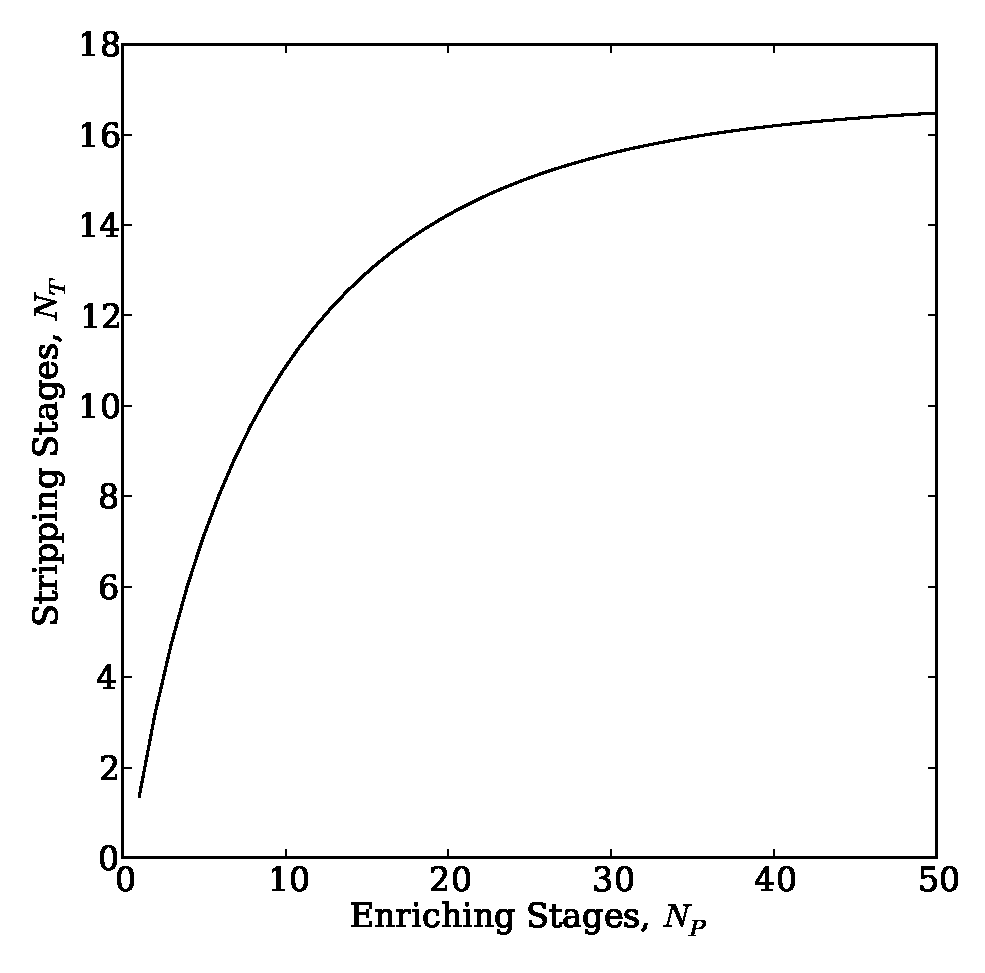
\includegraphics[scale=0.5]{nt_closed.eps}
\caption{$N_T(N_P, M^*)$ for a four component uranium re-enrichment cascade with 
         $N_P\in[1,50]$ and $M^*=236.547$.}
\label{nt_closed_fig}
\end{center}
\end{figure}

Figure \ref{nt_closed_fig} indicates that the closed form $N_T(N_P, M^*)$ is correct.
For an increasing number of enriching stages, the stripping stages must also 
increase to maintain the proper mass flow rates.
This data, and all remaining results, was computed 
with the feed concentrations in Table \ref{feed_vision}, 
$M^*=236.547$, $N_P^0=30$, $N_T^0=10$, $\alpha=1.05$, 
\nuc{U}{235} as the \jth key component, \nuc{U}{238} as the \kth key component, 
$x_j^P=0.055$, and $x_j^T=0.0025$.
Thus equation \ref{nt_closed} allows for the elimination of $N_T$ as an 
independent variable when computing $L/F$ and, more importantly here, $N_P$.  

\begin{table}[htbp]
\begin{center}
\caption{Feed flow concentrations for a four component uranium re-enichment cascade.}
\begin{tabular}{|l||c|}
\hline
\bf{Nuclide} & \bf{VISION $x^F$ \cite{Jacobson2009}} \\ 
\hline
U-234 & 0.00018 \\ 
\hline
U-235 & 0.00819 \\ 
\hline
U-236 & 0.00611 \\ 
\hline
U-238 & 0.98552 \\ 
\hline
\end{tabular}

\label{feed_vision}
\end{center}
\end{table}

Continuing on, the next MARC constraint is equation \ref{tail-constraint}.  
This maintains
the tails concentration of the second key component \emph{must} be equal to the 
concentration specified in the initial conditions.  
Substituting in the closed form solution of $N_T(N_P, M^*)$ above into the constraint, 
the function $f$ may be defined:
\begin{equation}
f(N_P,M^*) =
\left(\frac{x_j^F}{\frac{T}{F}} \cdot \frac{1 - \beta_i^{-N_P}}
                                           {\beta_j^{N_T(N_P,M^*)+1} - \beta_j^{-N_P}} \right)
- \left(x_j^T\cdot\sum_i^{I} x_i^T\right) \equiv 0
\label{fdefine}
\end{equation}
The simplified version of $T/F$ in equation \ref{tpf-key} is used here.  Note again
that there is no rearrangement of equation \ref{fdefine} that yields a $N_P$ as 
a function that does not include itself.  Roughly speaking this is due to the 
fact that $N_P$ occurs in equation \ref{fdefine} both in exponents of $\beta_i$ and
in exponents inside the $N_T$ substitiution, which iteself is in an exponent of 
$\beta_j$.  From Galois theory, these nested powers of $N_P$ imply that no closed form 
solution is possible.   Hence there is the need to approximate $f(N_P, M^*)$ and then
solve this in closed form for $N_P$.

\begin{figure}[htpb]
\begin{center}
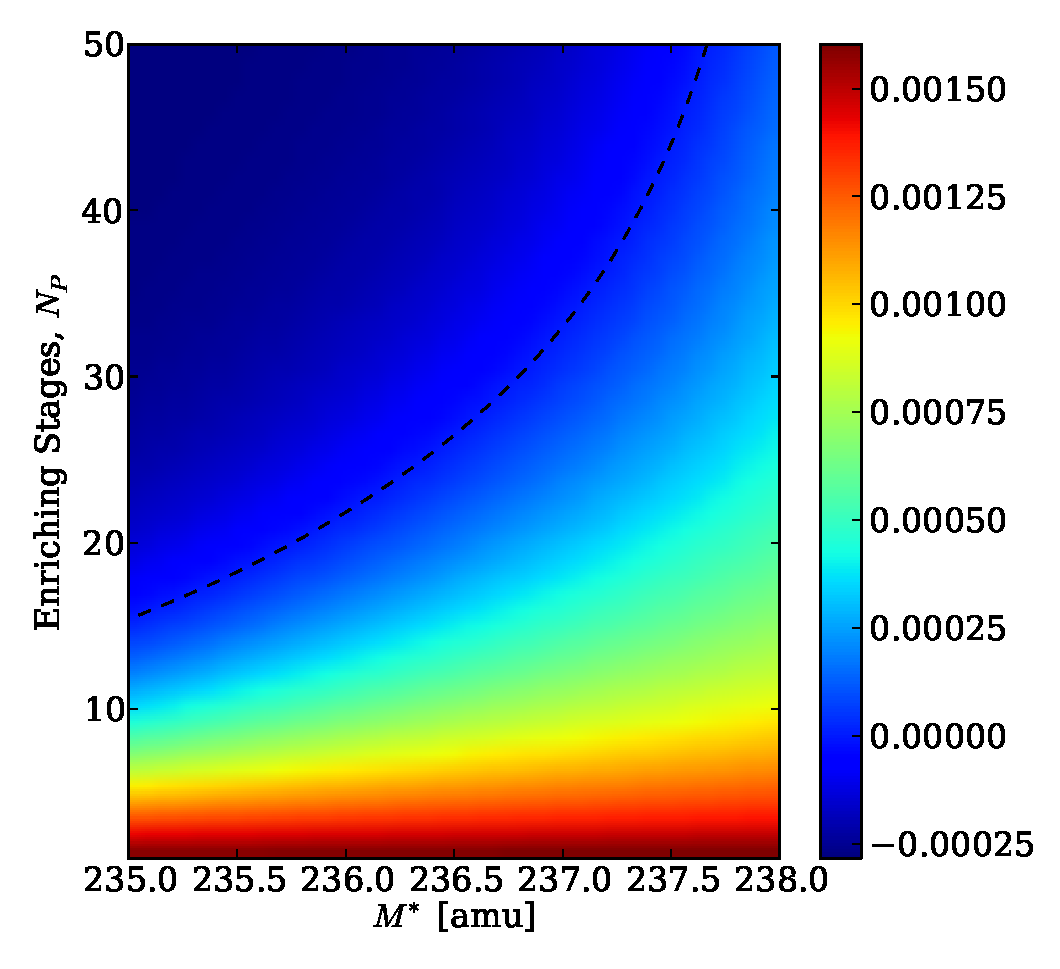
\includegraphics[scale=0.5]{np_constraint.eps}
\caption{$f(N_P, M^*)$ over the range of possible $N_P$ and $M^*$ values.  The black
dashed contour line represents $f(N_P, M^*)=0$ and is the solution to the MARC 
constraint in equation \ref{tail-constraint}. 
Data was computed for a four component uranium re-enrichment cascade.}
\label{np_constraint_fig}
\end{center}
\end{figure}

To gain a sense of the structure of this equation, $f(N_P,M^*)$ was plotted as an 
unconstrained function of $N_P$ and $M^*$.
This produces a heat map that may be seen in Figure \ref{np_constraint_fig}.  
Since the range of $f$ contains both positive and negative
values, it follows that there must be some combination of the independent variables 
which satisfies the $f\equiv 0$ constraint.  The solution curve $f(N_P, M^*)=0$ is 
also shown on Figure \ref{np_constraint_fig} as the black dashed contour.  
This contour could itself provide the closed form $N_P(M^*)$ equation.
However, this methodology be very computationally intensive and, thus, slow.  
This is due to the large number of $f$ points which would have to be 
computed interpolated create this curve.  This provides another justification as to 
why an upfront approximation method was used.

\subsection{Taylor Series Approximations}
\label{sec:aproxmeth}

The value of $f(N_P,M^*)=0$ in equation \ref{fdefine} was approximated using 
Taylor series expansions to first and second order.  These were then rearranged to 
$N_P(M^*)$, which is needed to eliminate $N_P$ from the MARC system.  
Due to the symbolic nature of the underlying algorithm, the coefficients in these
polynomial expansions cannot be precomputed numerically but must be 
expressed symbolically in terms of known parameters and independent variables 
\cite{Sacks:1989:ASS:1623755.1623823}.
Note that in 
either case, the approximation of $f$ should match the dashed countour line seen in 
Figure \ref{np_constraint_fig}, especially in the region near $M_0^*$.

From here, it is easy to represent $f$ by its first order Taylor series expansion
$f^{(1)}$ with respect to $N_P$ near the initial guess $N_P^0$.
\begin{equation}
f^{(1)}(N_P,M^*) \approx f(N_P^0,M^*) + 
    \left(N_P -N_P^0\right)\left.\frac{df}{dN_P}\right|_{N_P=N_P^0}
\label{f1-taylor}
\end{equation}
By setting equation \ref{f1-taylor} to zero and rearranging, it is easy to obtain the
closed form $N_P^{(1)}(M^*)$:
\begin{equation}
N_P^{(1)}(M^*) = N_P^0 - \frac{\left.\frac{df}{dN_P}\right|_{N_P=N_P^0}}{f(N_P^0,M^*)}
\label{np_closed1}
\end{equation}
The derivative in this equation is evaluated at initial guess $N_P^0$.
Note that this is equivalent to Newton's method for $N_P$.
Now for the second order Taylor series expansion, $f^{(2)}$, is as follows:
\begin{equation}
\begin{array}{rcl}
f^{(2)}(N_P,M^*) & \approx &f(N_P^0,M^*) \\
& & + \left(N_P -N_P^0\right)\left.\frac{df}{dN_P}\right|_{N_P=N_P^0} \\
& & + \frac{\left(N_P -N_P^0\right)^2}{2}\cdot\left.\frac{d^2f}{(dN_P)^2}\right|_{N_P=N_P^0}\\
\end{array}
\label{f2-taylor}
\end{equation}
Equation \ref{f2-taylor} may then be rearranged as a canonical polynomial form
with coefficients $a$, $b$, and $c$.
\begin{equation}
\begin{array}{rcl}
f^{(2)}(N_P,M^*) & = & a(N_P)^2 + bN_P + c\\
a & = & \frac{1}{2}\cdot\frac{d^2f}{(dN_P)^2}\\
b & = & \left.\frac{df}{dN_P}\right|_{N_P=N_P^0} - N_P^0\frac{d^2f}{(dN_P)^2} \\
c & = & f(N_P^0,M^*) - N_P^0\cdot\frac{df}{dN_P} + \frac{(N_P^0)^2}{2}\frac{d^2f}{(dN_P)^2} \\
\end{array}
\label{f-cannon}
\end{equation}
All derivatives are again evaluated at $N_P=N_P^0$.
Applying the constraint $f(N_P,M^*)=0$, 
a closed form expression $N_P(M^*)$ is trivially garnered by the 
quadratic equation.
\begin{equation}
N_P^{(2)}(M^*) = \frac{-b - \sqrt{b^2 - 4ac}}{2a}
\label{np_closed2}
\end{equation}
For the second order approximation $a$ must be positive, $b$ must be negative, 
and the discriminant is also positive.  Thus the 
negative root to the quadratic sufficient to to obtain a value of
$N_P^{(2)}(M^*)$ that is also positive and close to $N_P^0$.

\section{Approximation Results}
\label{sec:aproxres}

\begin{figure}[htpb]
\begin{center}
\begin{tabular}{cc}
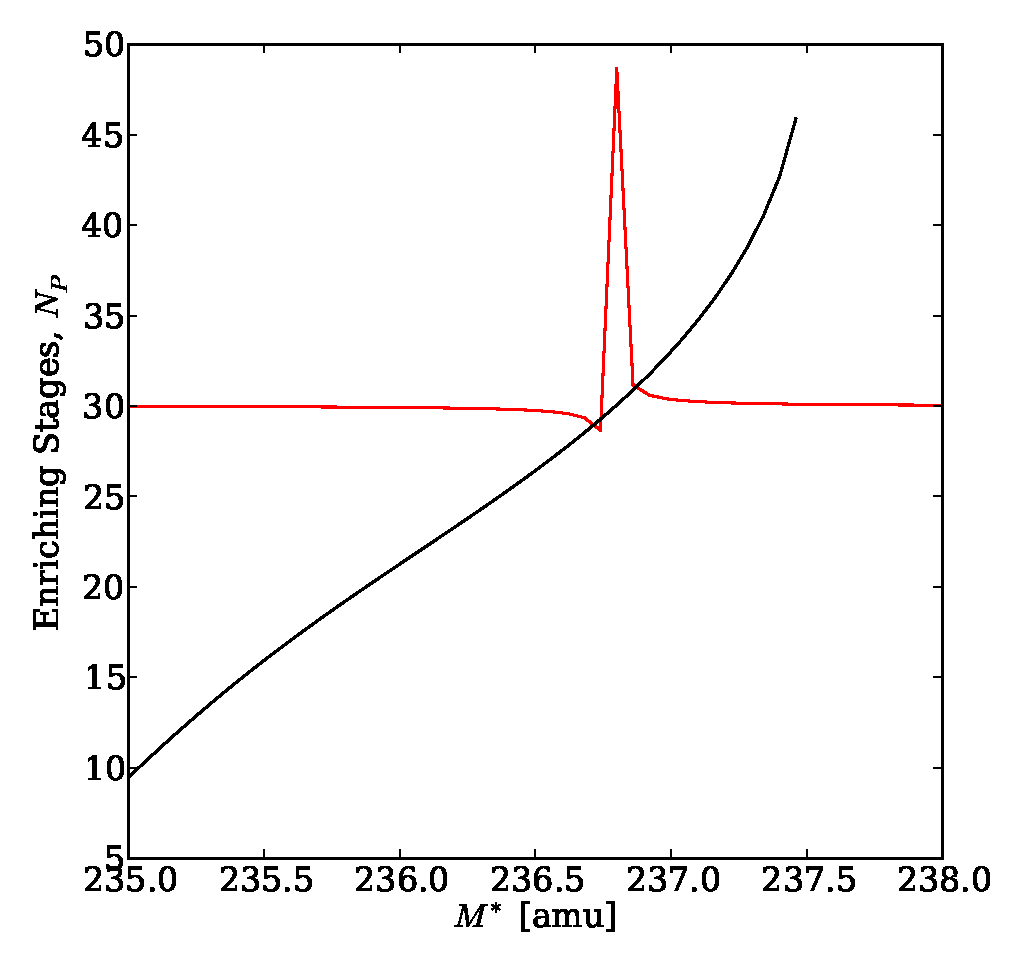
\includegraphics[scale=0.375]{np_closed.eps} & 
                                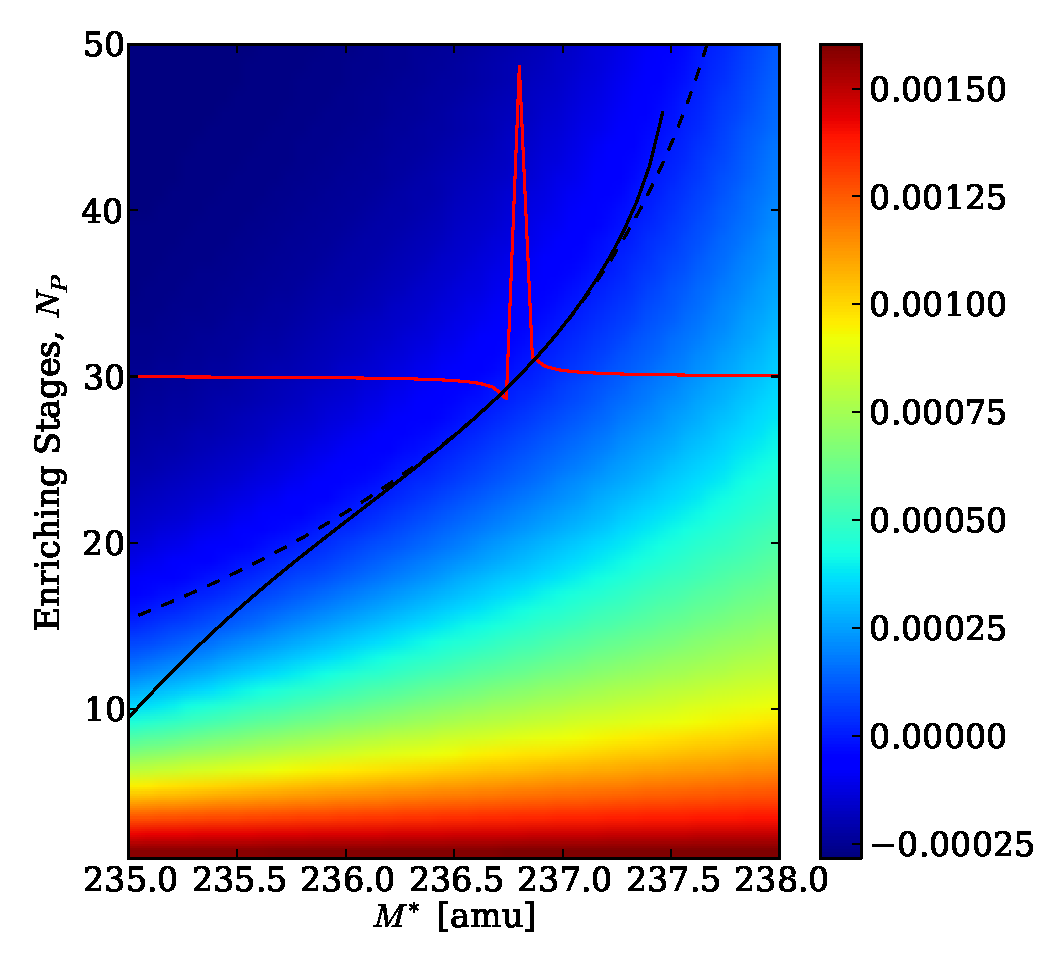
\includegraphics[scale=0.375]{np_closed_overlay.eps} \\
(a) & (b) \\
\end{tabular}
\caption{$N_P(M^*)$ such that $f(N_P,M^*)=0$.  (a): The solution to first and 
second order Taylor series approximations.  The first order curve is red while the 
second order curve is black. (b): The equations from (a) overlaid on top of Figure 
\ref{np_constraint_fig}.  The black dashed line is the contour at $f(N_P, M^*)=0$. 
Data was computed using a four component uranium re-enrichment cascade.}
\label{np_closed_fig}
\end{center}
\end{figure}

To qualify the validity of the first and second order approximations, 
Figure \ref{np_closed_fig} plots both closed form solutions to $N_P(M^*)$.
In Figure \ref{np_closed_fig}(a), these solutions are shown on their own.
In Figure \ref{np_closed_fig}(b) they are overlaid onto the heat map in 
Figure \ref{np_constraint_fig}.  

By inspection, the first order solution is almost wholly an inappropriate choice.
It stays quite near the initial guess for most portions of the domain.  As $M^*$
approaches $M_0^*$, the first order solution does cross the $f(N_P, M^*)=0$ curve 
and obtain the correct value.  However, at this point the first order approximation 
has the wrong sign on its slope.  This alone would make it inapproriate for 
use in a minimization calculation.  Furthermore, for larger values of $M^*$, an 
asymtotic-like peak and valley form.  This effectively gaurantees that any minimizer
would choose the wrong value.

On the other hand, the second order Taylor series approximation is very
accurate near the initial conditions.  As can be expected this approximation performs
less well for extreme values of $M^*$.  The second order solution over-predicts the 
result for the upper end of the domain and under-predicts for the lower end of the 
domain.  These discrepencies with $N_P^{(2)}(M^*)$ are expected Taylor series.

\begin{figure}[htpb]
\begin{center}
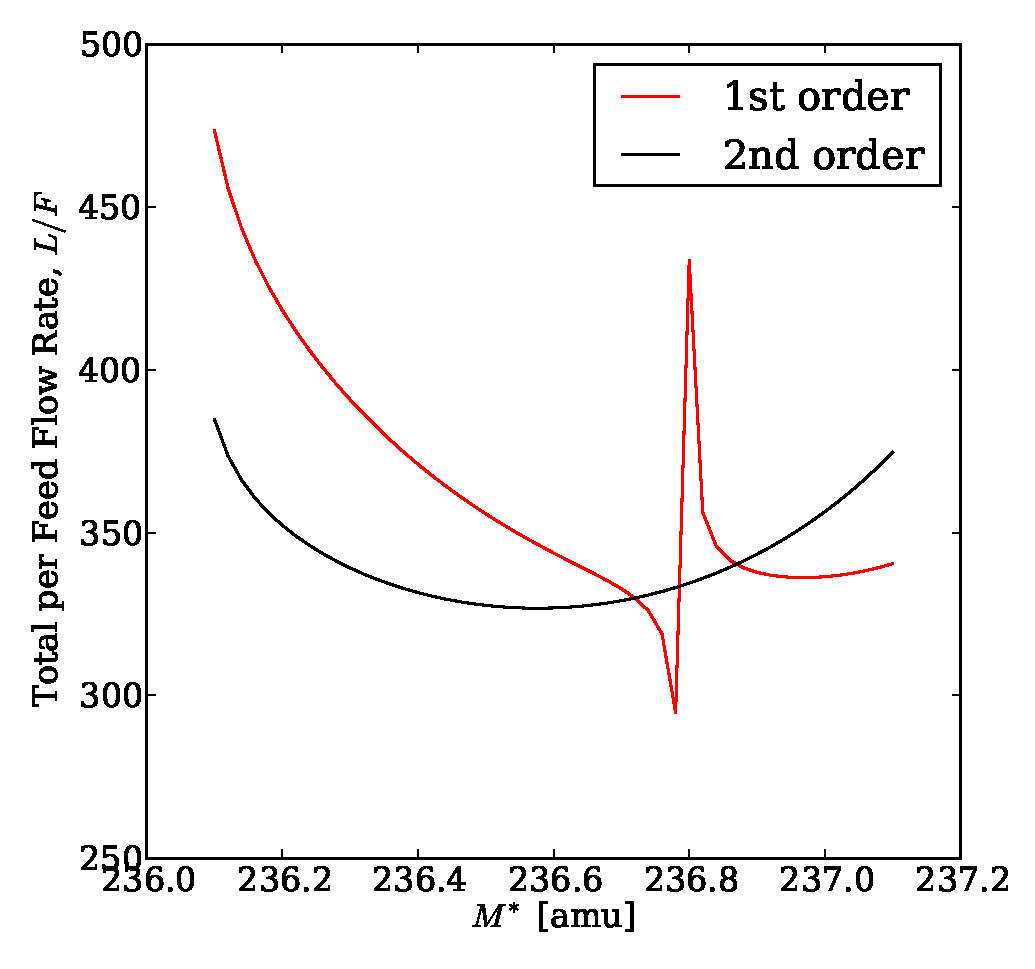
\includegraphics[scale=0.5]{loverf.eps}
\caption{$L/F(M^*)$ over the range of valid $M^*$ values.
Data was computed for a typical natural uranium cascade.}
\label{loverf_fig}
\end{center}
\end{figure}

Both equations \ref{np_closed1} \& \ref{np_closed2} may be substituted into 
equation \ref{nt_closed}.
Doing so will obtain an expressions $N_T(N_P(M^*),M^*)=N_T(M^*)$ which only depends on $M^*$ and 
the initial conditions.  Moreover, equations \ref{nt_closed} \& \ref{np_closed1} or 
equations \ref{nt_closed} \& \ref{np_closed2} could  then be substituted into 
equation \ref{ltot-over-feed}.   This would generate and expression 
$L/F(N_P(M^*),N_T(M^*),M^*)=L/F(M^*)$ only as a function of $M^*$.  From here it 
simple to minimze $L/F(M^*)$ using any one dimensional method.

In doing so
Figure \ref{loverf_fig} displays $L/F(M^*)$ for both the first and second order
approximations.  The second order method computes the proper bowl-like shape that is
expected.  This function may be easily minimized.  On the other hand, the asymtotic 
structure that was present in $N_P^{(1)}(M^*)$ is retained in the computation of 
$L/F(M^*)$.  Therefore, the first order approximation remains unacceptable when
solving for the minimum cascade.

\begin{table}[htbp]
\begin{center}
\caption{Number of instances of $M^*$ and the number of binary operations in 
         $L/F(M^*)$ for first and second order Taylor series approximations for a 
         four component mixture.}
\begin{tabular}{|l||c|c|}
\hline
& \bf{1st order} & \bf{2nd order} \\
\hline
No. $M^*$ & 6,852  &  111,012 \\ 
\hline
No. Ops   & 57,383 &  945,575 \\ 
\hline
\end{tabular}
\label{count_ops}
\end{center}
\end{table}


Note that while the second order Taylor series approximation is ultimately much more 
exact, the number of operations in the final form of $L/F(M^*)$ -- without the 
elimination of common terms -- is much larger than 
in the first order case.  Table \ref{count_ops} shows the counts the number of times
that $M^*$ appears in these expressions and the number of binary operations each 
takes to compute.  $M^*$ is included in this table as it is the only remaining 
independent variable.  The first order approximatzion contains about 6\% of the
$M^*$s that the second order version does.  Furthermore, the second order 
approximation has almost 16.5 times more operations than the first order 
approxiation.  Together these illustrate just how unfortunate it is that the first
order solution is not valid.  Luckily by eliminating common terms most of the 
performance edge of the first order can be regained in the second order solution
\cite{Scopatz2012}.

\section{Conclusions \& Future Work}
\label{sec:conc}

Given any system equations, it is often desirable to solve them via varibale 
elimination.  Unfortunately, closed form solutions for each independent variable
may not always be possible (see Galois theory).  In such cases, appoximations to 
the different variables may be used to obtain closed form solutions which are
adequately accurate.  However, the order to which these approximations are made
determines the validity of the overall solution.  This order is especially 
important if the system will be optimized.  However, there is a tension between 
the quality of the solution and how expensive it is to compute.

For the multicomponent MARC enrichment equations, the number of product stages 
required does not have a closed form solution.  Here instead afirst and second 
order Taylor series approximations were used.  The first order approximation 
yeilded and insufficent or incorect form over the entire domain.  However, 
the second order solution was very accurate over the domain of interest.  While 
the second order approximation deviated for extreme values of the domain, this 
tends not to matter as such domain values are not typically encountered.  
Therefore, it is recomended that all further computations use at least a second order
method.

Further work on the subject of approximating $N_P$ may include higher order Taylor
series approximations.  While these will likely give increasingly correct results 
for larger $M^*$ domains, it may not be the most efficient way to proceed.  
As these curves are smooth, other approximations may be chosen such as using 
radial basis functions, the Pade approximate, or Chebyshev rational approximations.

%\section*{References}
\setlength{\baselineskip}{12pt}

\bibliographystyle{ans}
\bibliography{refs}

\end{document}
